\subsection{Starbucks}
\subsubsection{Topologia estimada de red}
\begin{figure}[h!]
  \centering	
	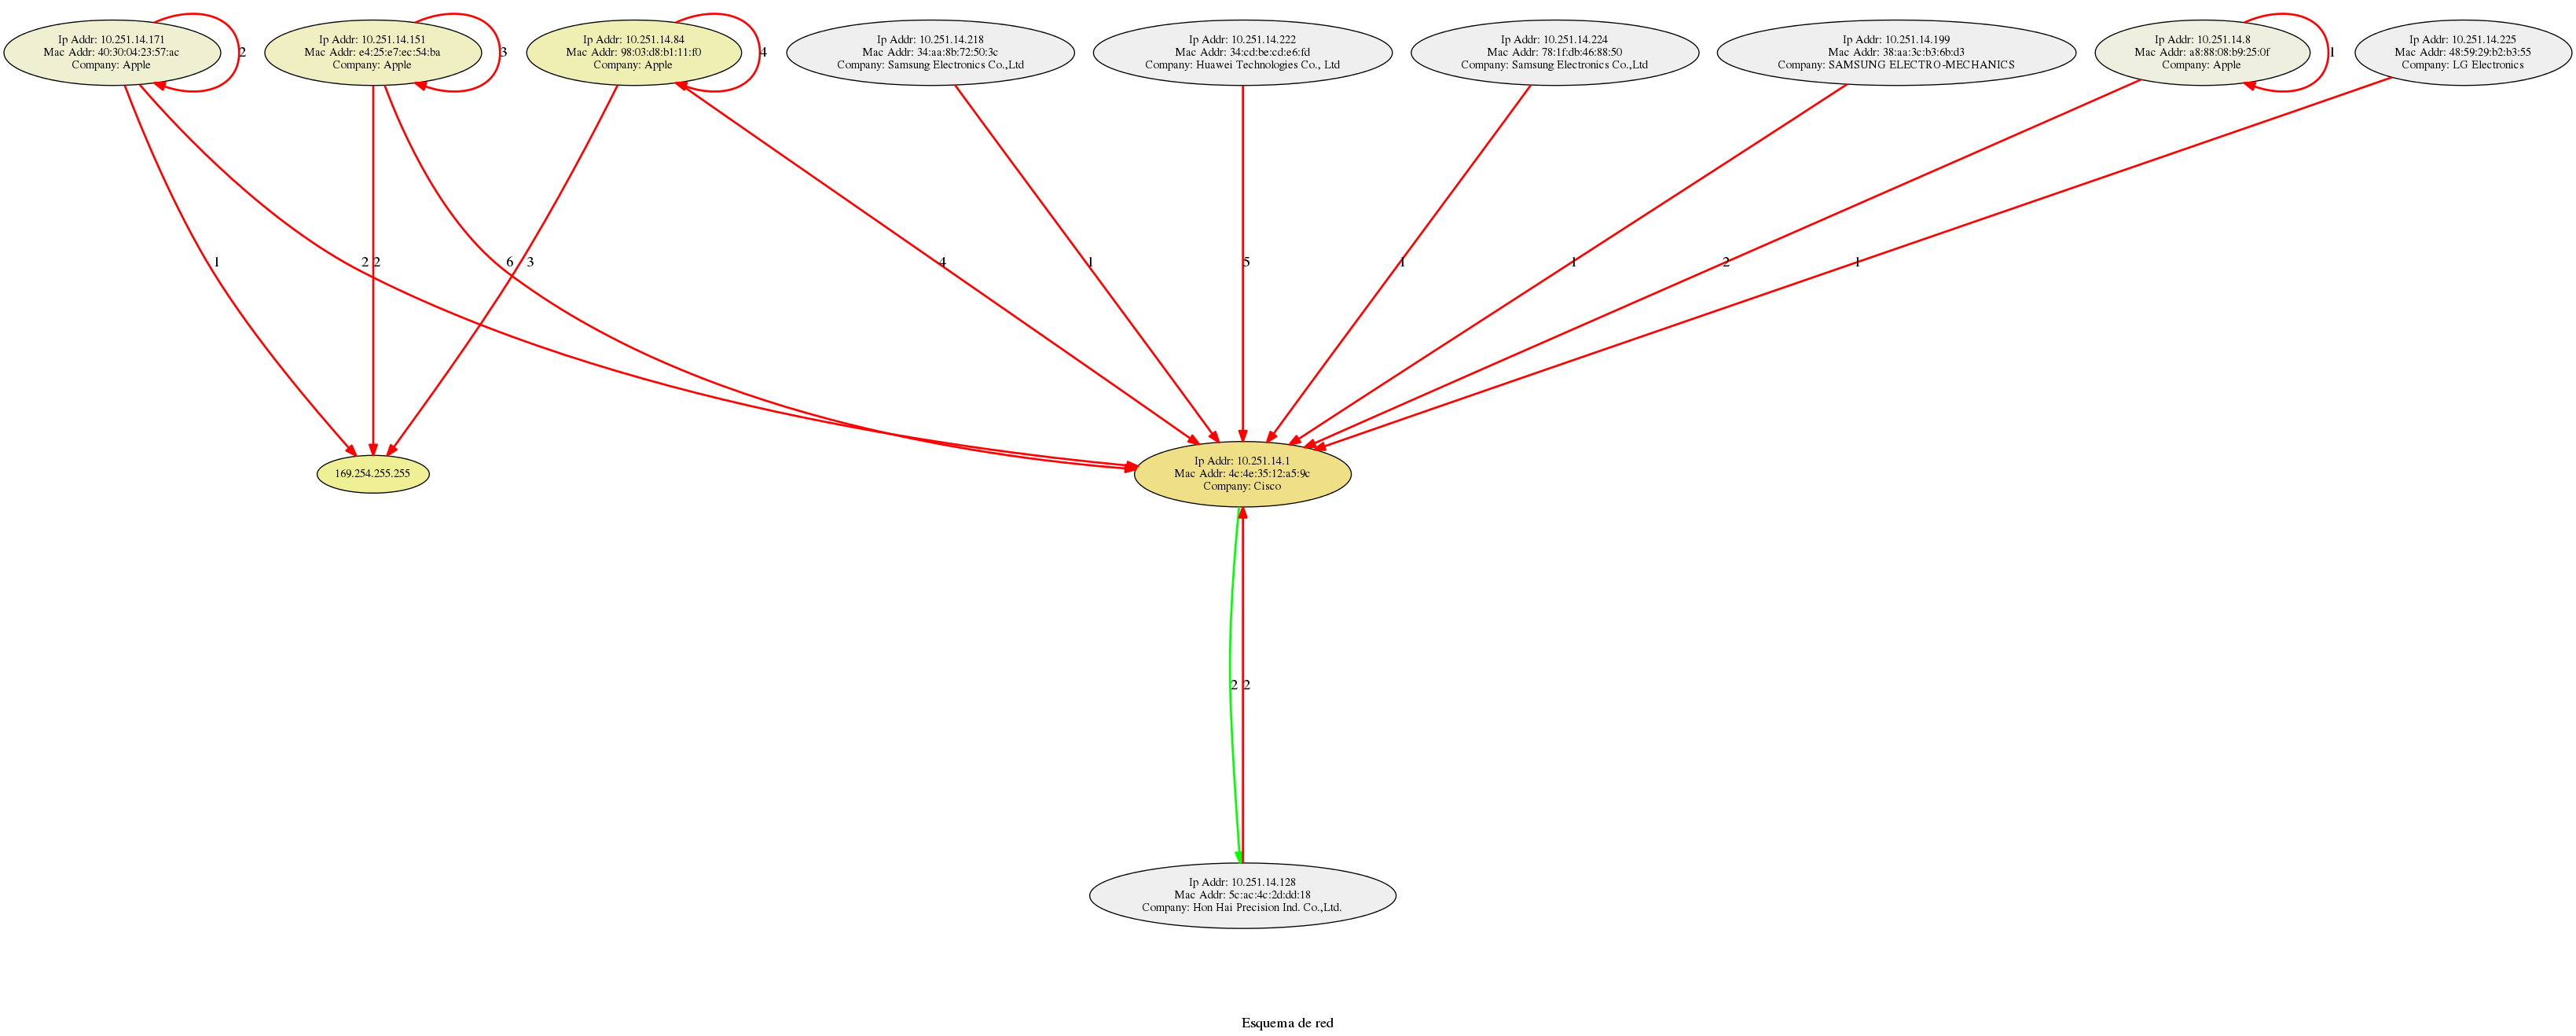
\includegraphics[scale=0.15]{../experimentacion-svilerino/starbucks/graph-starbucks-3.png}
  \caption{(grafo con experimento mas pequeño, el grafo completo puede encontrarse en la carpeta de experimentacion starbucks/full-experiment-1)}
  \label{fig:grafo-starbucks}
\end{figure}

\subsubsection{Probabilidades y entropia de fuente origen}
\begin{figure}[h!]
  \centering
	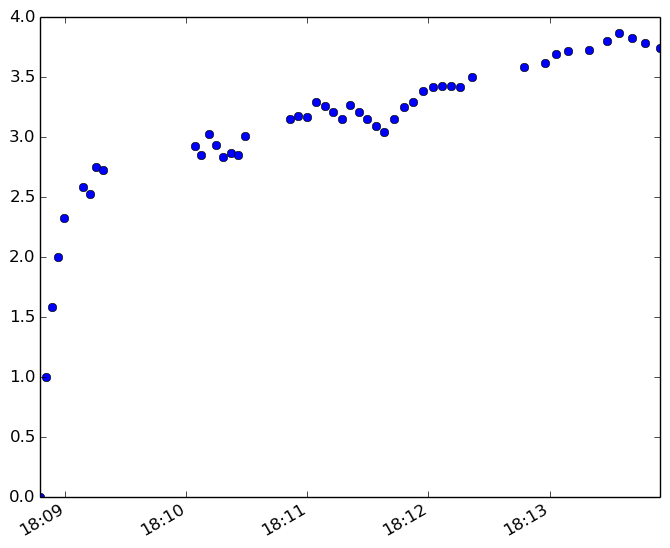
\includegraphics[scale=0.66]{../experimentacion-svilerino/starbucks/full-experiment-1/entropy_src.png}
  \caption{Entropia de la fuente origen.}
  \label{fig:entropia-src-starbucks}
\end{figure}

\begin{figure}[h!]
  \centering
	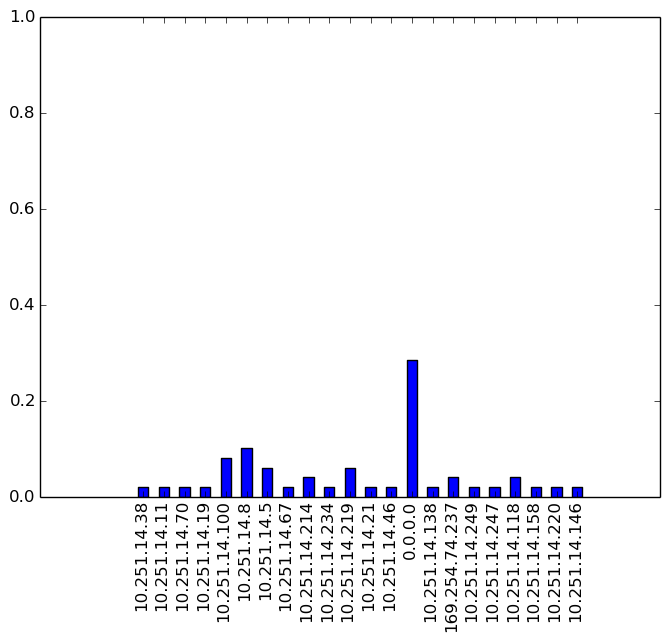
\includegraphics[scale=0.66]{../experimentacion-svilerino/starbucks/full-experiment-1/histogram_src_probabilities.png}
  \caption{Probabilidades asociadas a las IP de la fuente origen.}
  \label{fig:probabilidad-src-starbucks}
\end{figure}

%---------------------------------------------------------------------------------------------------------------

\subsubsection{Probabilidades y entropia de fuente destino}
\begin{figure}[h!]
  \centering
	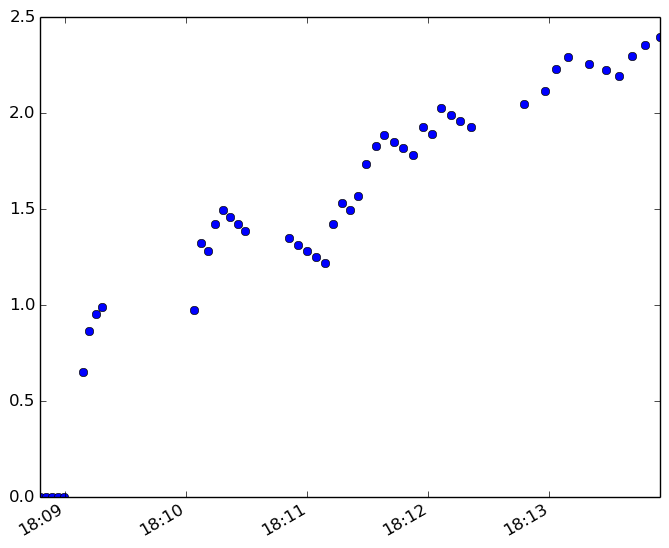
\includegraphics[scale=0.66]{../experimentacion-svilerino/starbucks/full-experiment-1/entropy_dst.png}
  \caption{Entropia de la fuente destino.}
  \label{fig:entropia-dst-starbucks}
\end{figure}

\begin{figure}[h!]
  \centering
	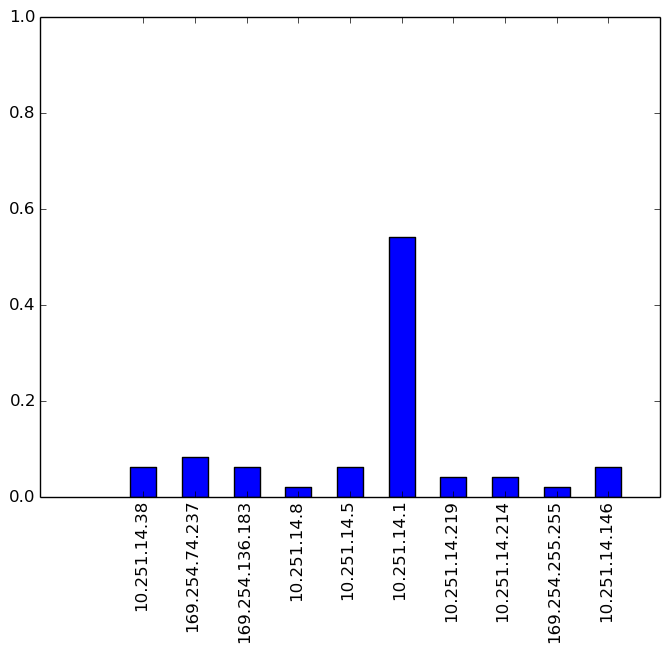
\includegraphics[scale=0.66]{../experimentacion-svilerino/starbucks/full-experiment-1/histogram_dst_probabilities.png}
  \caption{Probabilidades asociadas a las IP de la fuente destino.}
  \label{fig:probabilidad-dst-starbucks}
\end{figure}

\subsubsection{Tabla de dispositivos detectados}
\rowcolors{1}{Gray}{White}
\begin{tabular}{ |c|c|c| }
	\hline
	Ip Addr & Mac Addr & Company \\	
	\hline
	10.251.14.249 & 90:00:4e:80:fe:80 & Hon Hai Precision Ind. Co.,Ltd. \\
	\hline
	10.251.14.70 & 8c:3a:e3:0f:7f:88 & LG Electronics \\
	\hline
	169.254.74.237 & d8:9e:3f:d8:cd:96 & Apple \\
	\hline
	10.251.14.220 & c0:65:99:9b:a1:45 & Samsung Electronics Co.,Ltd \\
	\hline
	10.251.14.100 & b0:79:94:f8:ca:06 & Motorola Mobility LLC \\
	\hline
	10.251.14.138 & b4:3a:28:82:b6:45 & Samsung Electronics Co.,Ltd \\
	\hline
	10.251.14.247 & a8:06:00:2c:f1:0f & Samsung Electronics Co.,Ltd \\
	\hline
	10.251.14.234 & 18:26:66:ab:60:91 & Samsung Electronics Co.,Ltd \\
	\hline
	10.251.14.38 & 64:e6:82:b1:2b:d7 & Apple \\
	\hline
	10.251.14.46 & 70:aa:b2:4f:2b:1b & Research In Motion \\
	\hline
	10.251.14.214 & 48:9d:24:72:5b:ee & Research In Motion \\
	\hline
	10.251.14.19 & 00:e3:b2:ed:69:37 & Samsung Electronics Co.,Ltd \\
	\hline
	10.251.14.21 & d8:90:e8:2f:7d:1e & Samsung Electronics Co.,Ltd \\
	\hline
	10.251.14.5 & 00:25:d3:f6:1c:ec & AzureWave Technologies, Inc \\
	\hline
	10.251.14.67 & 40:6a:ab:3f:42:f9 & RIM \\
	\hline
	10.251.14.158 & 70:f9:27:ce:bb:e9 & Samsung Electronics \\
	\hline
	10.251.14.118 & 38:0b:40:05:ae:8f & Samsung Electronics Co.,Ltd \\
	\hline
	10.251.14.11 & f0:5a:09:ab:c9:1f & Samsung Electronics Co.,Ltd \\
	\hline
	0.0.0.0 & b0:35:8d:fa:d8:e0 & Nokia Corporation \\
	\hline
	10.251.14.8 & a8:88:08:b9:25:0f & Apple \\
	\hline
	10.251.14.219 & 48:9d:24:72:4f:d0 & Research In Motion \\
	\hline
\end{tabular}

\subsubsection{Conclusiones del experimento}
Este experimento se realizo sobre una red \textbf{no} controlada en una sucursal de \texttt{Starbucks}, los resultados obtenidos son relativamente los que se esperarian en una simple red abierta de \texttt{WiFi}. Puede observarse un nodo central y muchos hosts accediendo a el para obtener un servicio, en este caso \texttt{Internet}. Dado que luego de un tiempo muy corto el grafo comienza a ser poco claro dada la cantidad de hosts, el grafo mostrado en este informe es una version reducida(un experimento mas corto en tiempo), mientras que las estadisticas se sacaron con un experimento mas largo respecto al tiempo de escucha de la red. Nuevamente podemos inferir que el \texttt{access-point} de la red es el host \texttt{10.254.14.1} Dadas las figuras \ref{fig:grafo-starbucks} y \ref{fig:probabilidad-dst-starbucks}. Se observan ademas varios \href{http://wiki.wireshark.org/Gratuitous_ARP}{ARP gratuitos} en varios hosts de la figura \ref{fig:grafo-starbucks}. Como dato atipico adicional se observan pedidos a la direccion IP \texttt{169.254.255.255} que segun esta explicado en este sitio \url{http://packetlife.net/blog/2008/sep/24/169-254-0-0-addresses-explained/} podria deberse a no poder obtener una IP dinamicamente en la red y autoasignarse esta default IP. El resto de los hosts muestran un comportamiento estable. En consideracion respecto a las fuentes de informacion modeladas, podemos observar que nuevamente lo que pensamos es el \texttt{access-point} dado el fabricante \texttt{Cisco} en la IP \texttt{10.254.14.1} es el que con mas probabilidad es el destino de los paquetes \texttt{who-has} y el resto de los hosts reciben estos paquetes de forma mas equiprobable(aproximadamente). La entropia de la fuente destino va en aumento(creemos que va a estabilizarse luego de un tiempo) dado que observando el calculo de la entropia, los terminos de la suma se mantendran estable, salvo en del simbolo(IP) del \texttt{access-point} que seguira en aumento hasta cierto punto. Se observa similarmente en la fuente origen, que la entropia va en aumento, y tenemos una IP distinguida que aparece como origen \texttt{0.0.0.0}, observando la tabla de resolucion de dispositivos vemos que es un dispositivo del fabricante \texttt{Nokia Corporation}, asumimos que es algun dispositivo movil que no puede conectarse(e intenta muchas veces) el reenvio de paquetes a la red. Mas alla de esto el resto de las IPs(Simbolos) son mas equiprobables(aproximadamente) en la fuente origen por lo tanto creemos que la entropia ira en aumento hasta estabilizarse al este dispositivo lograr conectarse o dejar de intentar.